%----------------------------------------------------------------------------
\chapter{Inductive Shallow Node Embedding}
\label{sec:ISNE}
%----------------------------------------------------------------------------

\section{Problems with shallow encoders}
%----------------------------------------------------------------------------
In the previous chapter I presented the DeepWalk and node2vec algorithms for computing graph embeddings. They are both traditional shallow embedding methods, which rely on a lookup table encoder architecture.

Shallow Encoder Algorithms initially use a lookup table to represent nodes, where each node is assigned a unique embedding vector pre-defined in a low-dimensional space. This process, represented by the function $f$, essentially maps each node $v$ in the network to its corresponding embedding vector: ${f(v) = \Theta v}$.

However, algorithms employing lookup table encoders face two significant limitations:

\begin{enumerate}

    \item \emph{Transductivity:} node2vec and similar methods relying on lookup tables are inherently transductive. This means they cannot effectively generalize to unseen nodes that were not part of the training data. Consequently, their utility is restricted in scenarios involving dynamic networks or tasks necessitating predictions for new nodes.

    \item \emph{Static Embeddings:} the embeddings produced by node2vec are static; they do not dynamically update in response to changes in the network structure, such as edge additions or removals. This lack of adaptability poses challenges in real-world networks that frequently undergo dynamic alterations.

\end{enumerate}

These limitations make shallow embedding techniques unsuitable for tasks on continuously changing graphs, as even small changes in the graph can degrade the performance of the model significantly, and after more changes the model can easily become unusable. The static model cannot predict anything about new nodes. 

My task in this thesis is to implement a new dynamic encoder and compare it with the traditional encoder on different graph datasets by taking measurements. 

\section{Inductive Shallow Node Embedding}
%----------------------------------------------------------------------------

Inductive Shallow Node Embedding (ISNE) is a new dynamic graph embedding method proposed by $Richárd Kiss$ and $Gábor Szűcs$ in their paper [TODO cite]. ISNE employs an innovative encoder function designed to overcome the obstacles posed by both previously unseen nodes and dynamic network structures. This sophisticated design enables ISNE to:

\begin{itemize}
    \item \emph{Generalize to Unseen Nodes:} unlike transductive methodologies, ISNE is capable of effectively representing nodes that were not present during the training phase.
    \item \emph{Adapt to Dynamic Networks:} ISNE's representations can seamlessly adjust to modifications in the network structure, rendering them suitable for networks that evolve over time.
    \item \emph{Operate Independently of Node Attributes:} ISNE constructs embeddings exclusively based on the network's structure, thereby obviating the dependency on potentially unreliable or unavailable node attribute information.
\end{itemize}

Moreover, ISNE maintains the adaptability to incorporate node attributes by concatenating them to the existing ISNE embeddings. This feature allows users to harness the advantages of both network structure and node attributes, potentially yielding more robust and informative representations. Contrary to conventional shallow embedding techniques that rely on lookup tables, the proposed Inductive Shallow Node Embedding (ISNE) method utilizes a novel encoder function to construct node embeddings. This function operates based on the immediate neighbors of each node, as represented by the neighborhood set $N_v$. The fundamental update-step for the ISNE encoder is expressed in Equation~\ref{neigborhood}.

\clearpage

In this equation, ${h(v)}$ denotes the embedding vector of node 
$v$, with the summation iterating through all neighbors 
$n$ within its neighborhood set. This design ensures that a node's embedding is informed by the parameters of its immediate neighbors, effectively capturing the local network structure surrounding each node.

\begin{equation}
\label{neigborhood}
h(v) = \frac{1}{|N_v|} \sum_{n \in N_v} \theta_n
\end{equation}

This approach offers several critical advantages. Whenever a new edge is introduced to the network, the neighborhood set of the affected nodes (i.e., $N_j$ for specific nodes 
$j$) is updated accordingly. By recalculating ${h(v)}$ for these nodes, ISNE embeddings inherently reflect the latest structural changes within their local neighborhoods. The ISNE framework can generate embeddings for nodes that were previously unseen, provided their connections are known. By incorporating these connections into the neighborhood set during the encoding process (i.e., adding them to $N_v$ for the unseen node), ISNE can effectively estimate their embeddings.

This unique design also enables ISNE to perform inductive learning tasks. By relying solely on the network's structure and generalizing from existing information, the model can infer embeddings for unseen and modified data points, significantly enhancing its applicability in dynamic network settings and demonstrating adaptability to evolving graph structures.

In essence, the ISNE encoder transcends the limitations of traditional lookup tables by facilitating dynamic updates, accommodating unseen nodes, and supporting inductive learning tasks, thereby establishing itself as a critical tool for various network analysis applications.

\section{Comparison of different encoder result representations and theoretical representations}
%----------------------------------------------------------------------------

My task was to implement the new encoder (ISNE) and the node2vec algorithm, and then to train and evaluate the resulting models with different parameterizations on several data sets. I did a triple comparison, since I had to compare the similarity matrix derived from the embeddings of the two models with an implicit approximated and computed matrix. \cite{DBLP:journals/corr/abs-1710-02971} \cite{DBLP:journals/corr/YangL15} This matrices can be calculated both for DeepWalk and node2vec, using only the properties of the input graph and the hyperparameters used to teach it, as seen for DeepWalk in Equation~\ref{dw_M} and for node2vec Equation~\ref{n2v_M}

\begin{align}
\label{dw_M}
\log \left( {\text{vol}(G)} \left( \frac{1}{T} \sum_{r=1}^{T} \left( D^{-1}A \right)^r \right) D^{-1} \right) - \log b
\end{align}

\begin{align}
\label{n2v_M}
\log \left( \frac{1}{2T} \sum_{r=1}^{T} \left( \frac{\sum_{u} X_{w,u} P^{r}_{c,w,u} + \sum_{u} X_{c,u} P^{r}_{w,c,u}}{(\sum_{u} X_{w,u})(\sum_{u} X_{c,u})} \right) \right) - \log b
\end{align}

In the equations the following declarations were used \cite{DBLP:journals/corr/abs-1710-02971} \cite{DBLP:journals/corr/YangL15}:

\begin{itemize}
    \item \textbf{A:} $A \in \mathbb{R}_{+}^{|V| \times |V|}$ is $G$'s adjacency matrix with $A_{i,j}$ as the edge weight between vertices $i$ and $j$;
    \item \textbf{D\textsubscript{col}:} $D_{\text{col}} = \text{diag}(A^T e)$ is the diagonal matrix with the column sum of $A$;
    \item \textbf{D\textsubscript{row}:} $D_{\text{row}} = \text{diag}(Ae)$ is the diagonal matrix with the row sum of $A$;
    \item \textbf{D:} For undirected graphs $(A^T = A)$, $D_{\text{col}} = D_{\text{row}}$. For brevity, $D$ represents both $D_{\text{col}}$ and $D_{\text{row}}$. $D = \text{diag}(d_1, \ldots, d_{|V|})$, where $d_i$ represents the generalized degree of vertex $i$;
    \item \textbf{vol(G):} $\text{vol}(G) = \sum_{i} \sum_{j} A_{i,j} = \sum_{i} d_i$ is the volume of a weighted graph $G$;
    \item \textbf{T \& b:} The context window size and the number of negative sampling in skip-gram, respectively.
\end{itemize}

After calculating the implicit approximation of the matrices, I first compared the embeddings of node2vec using the traditional node2vec and the new decoder (ISNE). From the embeddings we can derive the similarity matrix interpreted on the vertices by taking the dot product of the embeddings with their transposed form. To calculate the similarity of the matrices, I used the following metrics:

\begin{enumerate}
    \item Using the Flatten function, I can get one-dimensional lists from the matrices, and plot two lists as a pair of points. Looking at this epoch by epoch, you can see that these points converge to the vicinity of the ${x=y}$ line. The closer they are to this line, the more similar the two similarity matrices, and hence the more similar the learned latent representations. Due to the large number of point pairs and their close proximity, I decided to use a heatmap to represent this.

    \item As in the previous point, the correlation coefficient between the two lists can be calculated. By calculating this for each epoch, we can plot the evolution of this coefficient during learning, ideally increasing it, since we expect that if we learn to convergence, the embeddings of the two models will be highly correlated.
\end{enumerate}

These methods can be used to show the degree of similarity of the matrices when comparing the three matrix sources. The measurements were made on several different sets of graph data, and with different hyperparameters during the training, which were naturally the same in the two models in a single measurement. Below are some visual results as examples, further results are detailed in the Appendix. Result of my first method shown on Figure~\ref{start_hm} and Figure~\ref{result_hm}. Figure~\ref{coef_res} displays the result of my second  method.

\begin{figure}[ht!]
	\centering
	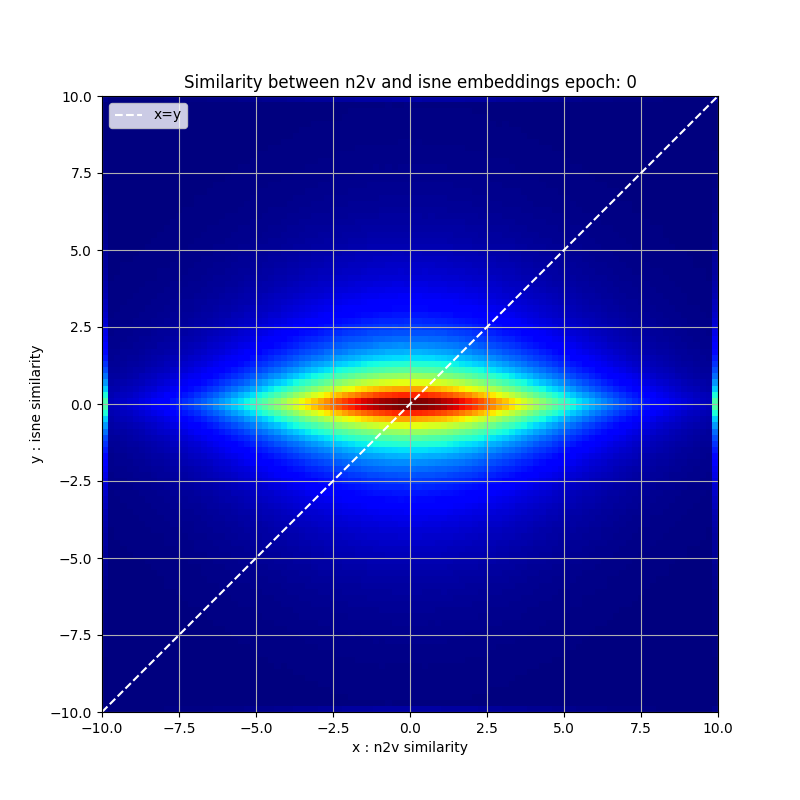
\includegraphics[width=0.70\textwidth]{figures/start_hm.png}
	\caption{On PubMed dataset, with ${p = 0.5, q =0.5}$ hiperparameters, initialization step, normalized noise.}
	\label{start_hm}
\end{figure}

\begin{figure}[ht!]
	\centering
	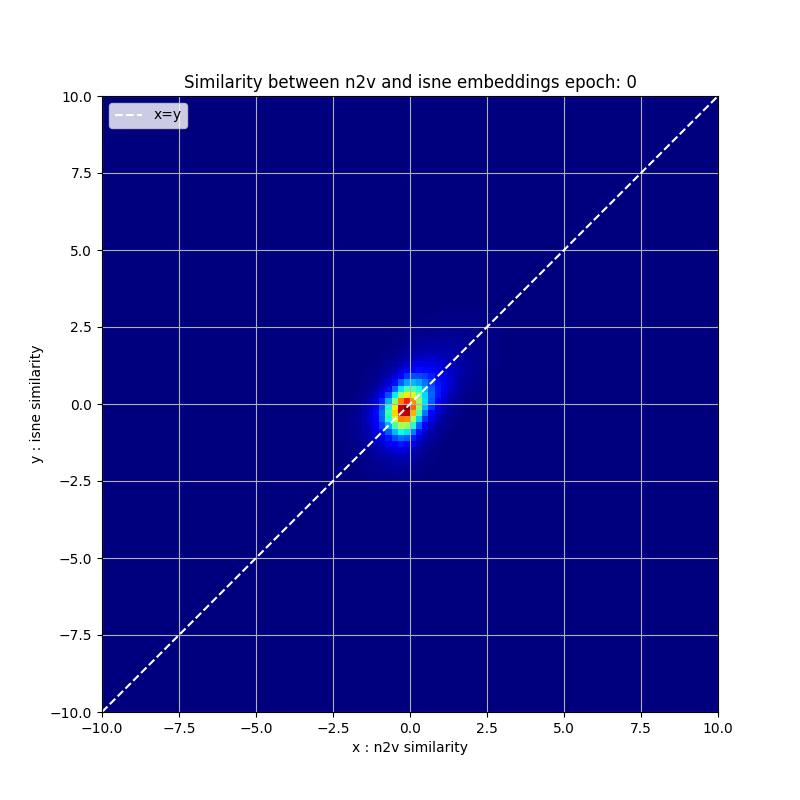
\includegraphics[width=0.70\textwidth]{figures/result_hm.png}
	\caption{On PubMed dataset, with ${p = 0.5, q =0.5}$ hiperparameters, after 40. epoch.}
	\label{result_hm}
\end{figure}

\begin{figure}[ht!]
	\centering
	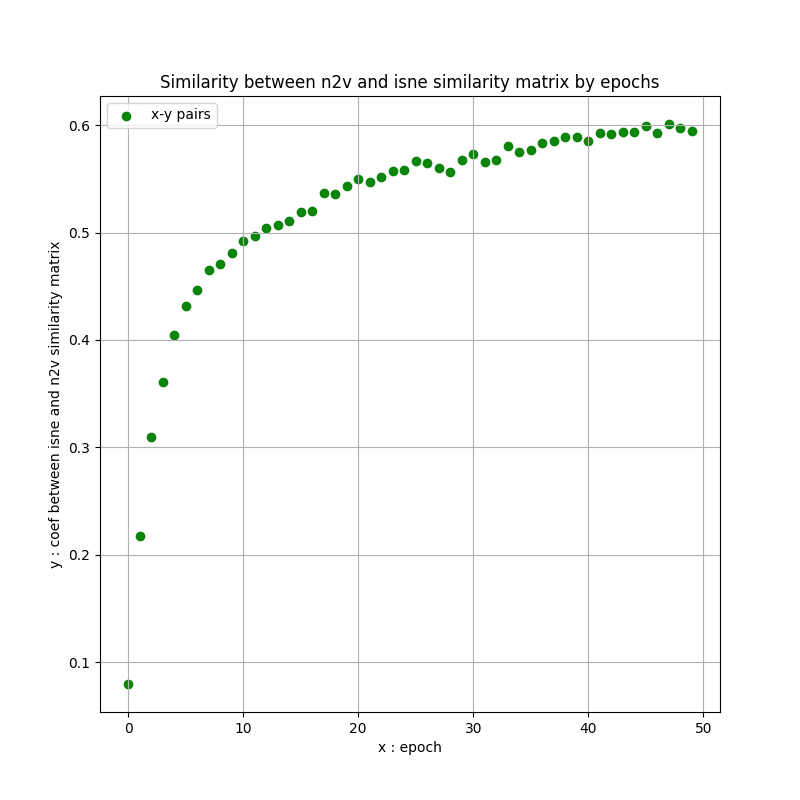
\includegraphics[width=0.70\textwidth]{figures/Cora_05_05_coef_plot.png}
	\caption{On PubMed dataset, with ${p = 0.5, q =0.5}$ hiperparameters, correlation coef through 50 epoch.}
	\label{coef_res}
\end{figure}